\documentclass[a4paper,12pt]{article}

\documentclass[a4paper,12pt]{article}

\usepackage{indentfirst}
\usepackage{cite}
\usepackage[utf8]{inputenc}
\usepackage[T1]{polski}
\usepackage{helvet}
\usepackage{graphicx}
\usepackage{svg}
\usepackage{color}
\usepackage{geometry}
\usepackage{float}
\usepackage{multirow}
\usepackage[hidelinks]{hyperref}
\usepackage{caption}
% dodaj bibliografię do spisu treści
\usepackage[nottoc]{tocbibind}
% unikaj pojedynczych linii na początku/ końcu stron
\usepackage[defaultlines=4,all]{nowidow}
\usepackage{subcaption}
\usepackage{amsmath}
\usepackage{amsfonts}

% set default figure placement to !htbp
\makeatletter
\def\fps@figure{!htbp}
\makeatother


\newcommand{\setSubtitle}[1]{
    \newcommand{\subtitle}{#1}
    }

\newcommand{\labdate}{25 listopada 2020}
\newcommand{\temat}{Właściwości sprężyste}

\begin{document}
    
% Please add the following required packages to your document preamble:
% \usepackage{multirow}
% \usepackage{graphicx}

\begin{table}[]
    \resizebox{\textwidth}{!}{%
    \begin{tabular}{|c|c|c|c|}
    \hline
    \multicolumn{2}{|c|}{\multirow{2}{*}{\hspace{0.5cm} 
\includegraphics[height=2.3cm]{img/logoAGH} \hspace{0.5cm} }}                                                                    & \multicolumn{2}{c|}{\textbf{\begin{tabular}[c]{@{}c@{}} Akademia Górniczo-Hutnicza w Krakowie\\ Wydział Inżynierii Materiałowe i Ceramiki  \vspace{0.5cm} \end{tabular}}}                                     \\ \cline{3-4} 
    \multicolumn{2}{|c|}{}                                                                                       & \multicolumn{2}{c|}{\begin{tabular}[c]{@{}c@{}}Aleksandra Barcz\\ Alicja Kotwica  \vspace{0.5cm} \end{tabular}}                                                                                              \\ \hline
    \multicolumn{4}{|c|}{\textbf{Metody Badań Materiałów}}                                                                                                                                                                                                                                                     \\ \hline
    \multicolumn{4}{|c|}{\textbf{\temat}}                                                                                                                                                                                                                                                                            \\ \hline
    \begin{tabular}[c]{@{}c@{}}Rok Akademicki:\\ 2020/2021\end{tabular}         & \multicolumn{2}{c|}{\begin{tabular}[c]{@{}c@{}}Rok studiów:\\ IV\end{tabular}}                                  & \begin{tabular}[c]{@{}c@{}}Kierunek:\\ Ceramika\end{tabular}                                                       \\ \hline
    \begin{tabular}[c]{@{}c@{}}Data wykonania ćwiczenia\\ \labdate \end{tabular} & \multicolumn{2}{c|}{\begin{tabular}[c]{@{}c@{}}Data oddania sprawozdania:\\ \today \end{tabular}} & \begin{tabular}[c]{@{}c@{}}Prowadzący:\\ Dr. inż. Beata Macherzyńska\end{tabular}                                  \\ \hline
    \end{tabular}%
    }
    \end{table}


\section{Cel ćwiczenia}

Celem ćwiczenia było zapoznanie się  metoda cienia (przepuszczania) oraz wyznaczanie modułów Younga, Kirhoffa oraz liczby Poissona dla materiałów izotropowych.

\section{Wprowadzenie}

Jedną z~metod ultradźwiękowych jest metoda cienia (przepuszczania). Metoda ta polega na wprowadzeniu fal ultradźwiękowych z~jednej strony badanego materiału i~odbieraniu ich z~drugiej strony po przejściu przez materiał, podczas obserwacji natężenia fal przechodzących. Każda wada w~badanym materiale odbija falę ultradźwiękową tworząc tak jakby cień, zatem fala przechodząca jest osłabiona i~głowica odbiorcza odbiera falę o~mniejszej intensywności.

W~metodzie używa się dwóch takich samych głowic ustawionych prostopadle (najczęściej) lub skośnie. Sygnał prowadzonych z~głowicy odbiorczej do detektora, a~z~niego do lampy oscyloskopowej. Obecność wady można zauważyć poprzez zmianę sygnału odbieranego przez głowice odbiorczą.

Wadą tej metody jet niemożliwe określenia położenia wady. Dodatkowo takie same wady, będące w~innych miejscach próbki będą inaczej osłabiać wiązkę fal ultradźwiękowych na skutek tworzenia się cienia. Kolejną wadą jest konieczność ustawiania głowic centrycznie. Zaletą tej metody jest wykrywanie wad blisko powierzchni materiału wad, które są różnie zorientowane w~przestrzeni.
\newline

Źródło: Materiały otrzymane przez prowadzącego "Metody Badań, Badania Ultradźwiękowe" dr. Jan Piekarczyk

\section{Aparatura i~materiały}

Aparatura:

\begin{itemize}
    \item defektoskop ultradźwiękowy  DI-40
    \item ośrodki sprzęgające: olej do fal podłużnych i~balsam kanadyjski do fal poprzecznych.
    \item suwmiarka
    \item waga analityczna
    \item głowica normalna do fal podłużnych $10LO^\circ10C$
    \item głowica skośna do fal poprzecznych 3T
\end{itemize} 
 
 Materiały:
 
 \begin{itemize}
     \item wzorzec stalowy $2\mu s$
     \item $Al_2O_3$ sześcian 
     \item $Al_2O_3$ prostopadłościan krótki
     \item $Al_2O_3$ prostopadłościan długi 
     \item SiC
     \item $ZrO_2$
     \item Żywica epoksydowa 
     \item Stal 
 \end{itemize}
\newpage
 
\section{Wyniki i~obliczenia}

\subsection{Wyznaczanie gęstości próbek}

Zmierzyliśmy suwmiarką oraz zważyliśmy na wadze otrzymane próbki, przedstawione na schematach poniżej. Otrzymane wielkości i~masę zapisaliśmy w~tabeli 1. 
Na podstawie tych pomiarów policzyliśmy objętość i~gęstość badanych materiałów.

\begin{figure}[H]
    \centering
    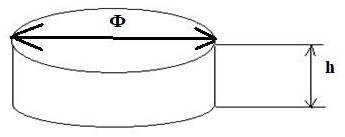
\includegraphics[width=0.5\textwidth]{img/wzorzec.jpg}
    \caption{Schemat wzorca stalowego $2$ $\mu s$.}
\end{figure}

\begin{figure}[H]
    \centering
    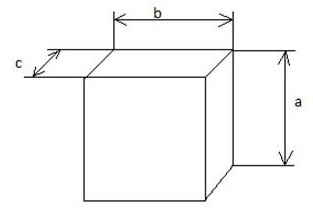
\includegraphics[width=0.6\textwidth]{img/szescianAl2O3_SiC.jpg}
    \caption{Schemat sześcianu $Al_2O_3$.}
\end{figure}

\begin{figure}[H]
    \centering
    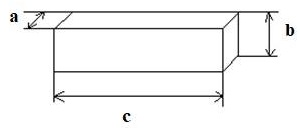
\includegraphics[width=0.7\textwidth]{img/krotkiAl2O3.jpg}
    \caption{Schemat prostopadłościanu krótkiego $Al_2O_3$.}
\end{figure}

\begin{figure}[H]
    \centering
    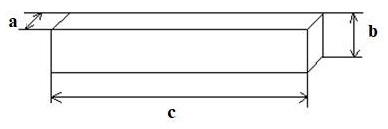
\includegraphics[width=0.7\textwidth]{img/dlugiAl2O3_stal.jpg}
    \caption{Schemat prostopadłościanu długiego $Al_2O_3$.}
\end{figure}

\begin{figure}[H]
    \centering
    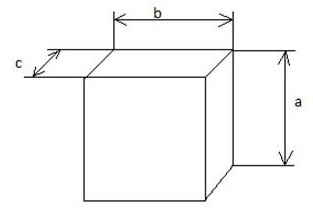
\includegraphics[width=0.6\textwidth]{img/szescianAl2O3_SiC.jpg}
    \caption{Schemat $SiC$.}
\end{figure}

\begin{figure}[H]
    \centering
    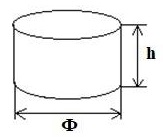
\includegraphics[width=0.5\textwidth]{img/ZrO2.jpg}
    \caption{Schemat $ZrO_2$.}
\end{figure}

\begin{figure}[H]
    \centering
    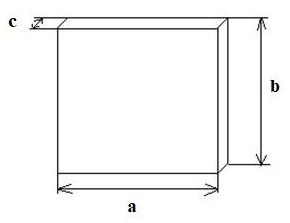
\includegraphics[width=0.6\textwidth]{img/zywica.jpg}
    \caption{Schemat żywicy epoksydowej.}
\end{figure}

\begin{figure}[H]
    \centering
    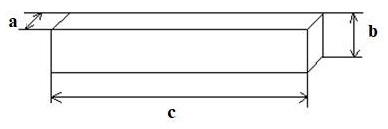
\includegraphics[width=0.7\textwidth]{img/dlugiAl2O3_stal.jpg}
    \caption{Schemat stali.}
\end{figure}

% Please add the following required packages to your document preamble:
% \usepackage{graphicx}
\begin{table}[H]
    \centering
    \caption{Zestawienie wymiarów, masy oraz gęstości dla wzorców oraz próbek}
    \label{tab:my-table}
    \resizebox{\textwidth}{!}{%
    \begin{tabular}{|c|r|r|r|r|r|r|}
    \hline
    Nazwa próbki                                                                 & \multicolumn{1}{c|}{\begin{tabular}[c]{@{}c@{}}Długość (a) / \\ średnica ($\Phi$) \\ $[cm]$\end{tabular}} & \multicolumn{1}{c|}{\begin{tabular}[c]{@{}c@{}}Szerokość (b) \\ $[cm]$\end{tabular}} & \multicolumn{1}{c|}{\begin{tabular}[c]{@{}c@{}}Grubość (c) / \\ wysokość (h) \\ $[cm]$\end{tabular}} & \multicolumn{1}{c|}{Masa $[g]$} & \multicolumn{1}{c|}{\begin{tabular}[c]{@{}c@{}}Objętość \\ $[cm^3]$\end{tabular}} & \multicolumn{1}{c|}{\begin{tabular}[c]{@{}c@{}}$\rho$ \\ $[g/cm^3]$\end{tabular}} \\ \hline
    Wzorzec $2\mu s$                                                             & 4.00                                                                                                      & -                                                                                    & 1.15                                                                                                 & 118.1685                        & 14.44                                                                             & 8.18                                                                              \\ \hline
    $Al_2O_3$ sześcian                                                           & 2.00                                                                                                      & 2.00                                                                                 & 2.00                                                                                                 & 30.3169                         & 8.00                                                                              & 3.79                                                                              \\ \hline
    \begin{tabular}[c]{@{}c@{}}$Al_2O_3$ \\ prostopadłościan krótki\end{tabular} & 1.30                                                                                                      & 1.90                                                                                 & 4.90                                                                                                 & 41.9354                         & 12.10                                                                             & 3.46                                                                              \\ \hline
    \begin{tabular}[c]{@{}c@{}}$Al_2O_3$ \\ prostopadłościan długi\end{tabular}  & 1.25                                                                                                      & 1.95                                                                                 & 9.90                                                                                                 & 93.6573                         & 24.13                                                                             & 3.88                                                                              \\ \hline
    $SiC$                                                                        & 5.10                                                                                                      & 5.10                                                                                 & 1.20                                                                                                 & 92.9754                         & 31.21                                                                             & 2.98                                                                              \\ \hline
    $ZrO_2$                                                                      & 1.65                                                                                                      & -                                                                                    & 1.00                                                                                                 & 12.1778                         & 2.14                                                                              & 5.70                                                                              \\ \hline
    Żywica epoksydowa                                                            & 2.35                                                                                                      & 2.45                                                                                 & 1.80                                                                                                 & 12.3012                         & 10.36                                                                             & 1.19                                                                              \\ \hline
    Stal                                                                         & 2.38                                                                                                      & 3.85                                                                                 & 14.65                                                                                                & -                               & 134.24                                                                            & -                                                                                 \\ \hline
    \end{tabular}%
    }
    \end{table}

\subsection{Wyznaczanie prędkości propagacji podłużnej fali ultradźwiękowej $(C_L)$}

Zgodnie z~instrukcją ustawiono defektoskop na pomiar drogi przy zastosowaniu fali podłużnej. Przy użyciu dwóch głowic $10LO^\circ10C$ ustawionych jednoosiowo (jedna z~nich została umieszczona na statywie, a~drugą umieszczono tak, aby zachować jednoosiowość), przeprowadzono pomiar dla poszczególnych kierunków w~każdej próbce. Podczas pomiaru dla fali podłużnej używano oleju. Otrzymane wyniki pomiarów zamieszczono w~tabeli 2.

Posiadając pomiary długości fali obliczyliśmy wartości średnie czasu i~odchylenie standardowe każdej z~próbek, w~każdym kierunku pomiarowym. Wyniki obliczeń również podaliśmy w~tabeli 2.

% Please add the following required packages to your document preamble:
% \usepackage{multirow}
% \usepackage{graphicx}
\begin{table}[H]
    \centering
    \caption{Zestawienie wyników pomiarów czasu przejścia fali podłużnej $t_L$.}
    \label{tab:my-table}
    \resizebox{0.8\textwidth}{!}{%
    \begin{tabular}{|c|c|r|r|r|r|}
    \hline
    \multicolumn{2}{|c|}{Próbka}                                                                                & \multicolumn{1}{c|}{$t_1 [\mu s]$} & \multicolumn{1}{c|}{$t_2 [\mu s]$} & \multicolumn{1}{c|}{$t_{sr} [\mu s]$} & \multicolumn{1}{c|}{$\sigma _t [\mu s]$} \\ \hline
    \multirow{5}{*}{\begin{tabular}[c]{@{}c@{}}Wzorzec \\ $2\mu s$\end{tabular}}                     & 1 impuls & 7                                  & 6                                  & 6.5                                   & 0.7                                      \\ \cline{2-6} 
                                                                                                     & echo 1   & 19                                 & 19                                 & 19.0                                  & 0.0                                      \\ \cline{2-6} 
                                                                                                     & echo 2   & 31                                 & 32                                 & 31.5                                  & 0.7                                      \\ \cline{2-6} 
                                                                                                     & echo 3   & 43                                 & 44                                 & 43.5                                  & 0.7                                      \\ \cline{2-6} 
                                                                                                     & echo 4   & 56                                 & 56                                 & 56.0                                  & 0.0                                      \\ \hline
    \multirow{3}{*}{\begin{tabular}[c]{@{}c@{}}$Al_2O_3$ \\ sześcian\end{tabular}}                   & a        & 6                                  & 6                                  & 6.0                                   & 0.0                                      \\ \cline{2-6} 
                                                                                                     & b        & 6                                  & 6                                  & 6.0                                   & 0.0                                      \\ \cline{2-6} 
                                                                                                     & c        & 6                                  & 6                                  & 6.0                                   & 0.0                                      \\ \hline
    \multirow{3}{*}{\begin{tabular}[c]{@{}c@{}}$Al_2O_3$ \\ prostopadłościan \\ krótki\end{tabular}} & a        & 5                                  & 5                                  & 5.0                                   & 0.0                                      \\ \cline{2-6} 
                                                                                                     & b        & 7                                  & 7                                  & 7.0                                   & 0.0                                      \\ \cline{2-6} 
                                                                                                     & c        & 17                                 & 17                                 & 17.0                                  & 0.0                                      \\ \hline
    \multirow{3}{*}{\begin{tabular}[c]{@{}c@{}}$Al_2O_3$ \\ prostopadłościan \\ długi\end{tabular}}  & a        & 5                                  & 5                                  & 5.0                                   & 0.0                                      \\ \cline{2-6} 
                                                                                                     & b        & 6                                  & 6                                  & 6.0                                   & 0.0                                      \\ \cline{2-6} 
                                                                                                     & c        & 30                                 & 30                                 & 30.0                                  & 0.0                                      \\ \hline
    \multirow{3}{*}{$SiC$}                                                                           & a        & 14                                 & 14                                 & 14.0                                  & 0.0                                      \\ \cline{2-6} 
                                                                                                     & b        & 14                                 & 14                                 & 14.0                                  & 0.0                                      \\ \cline{2-6} 
                                                                                                     & c        & 4                                  & 3                                  & 3.5                                   & 0.7                                      \\ \hline
    \multirow{2}{*}{$ZrO_2$}                                                                         & $\Phi$   & 8                                  & 8                                  & 8.0                                   & 0.0                                      \\ \cline{2-6} 
                                                                                                     & h        & 5                                  & 5                                  & 5.0                                   & 0.0                                      \\ \hline
    \multirow{3}{*}{\begin{tabular}[c]{@{}c@{}}Żywica \\ epoksydowa\end{tabular}}                    & a        & 25                                 & 25                                 & 25.0                                  & 0.0                                      \\ \cline{2-6} 
                                                                                                     & b        & 27                                 & 27                                 & 27.0                                  & 0.0                                      \\ \cline{2-6} 
                                                                                                     & c        & 20                                 & 20                                 & 20.0                                  & 0.0                                      \\ \hline
    \multirow{3}{*}{Stal}                                                                            & a        & 13                                 & 12                                 & 12.5                                  & 0.7                                      \\ \cline{2-6} 
                                                                                                     & b        & 21                                 & 20                                 & 20.5                                  & 0.7                                      \\ \cline{2-6} 
                                                                                                     & c        & 74                                 & 74                                 & 74.0                                  & 0.0                                      \\ \hline
    \end{tabular}%
    }
    \end{table}

% Please add the following required packages to your document preamble:
% \usepackage{multirow}
% \usepackage{graphicx}
\begin{table}[H]
    \centering
    \caption{Zestawienie wartości średnich czasu przejścia fali podłużnej $t_{Lsred}$ oraz odległości między echami $\theta$ dla wzorca.}
    \label{tab:my-table}
    \resizebox{0.7\textwidth}{!}{%
    \begin{tabular}{|c|c|r|r|r|r|r|}
    \hline
    \multicolumn{2}{|c|}{Próbka}                                                            & \multicolumn{1}{c|}{\begin{tabular}[c]{@{}c@{}}$t_{sr}$ \\ $[\mu s]$\end{tabular}} & \multicolumn{1}{c|}{\begin{tabular}[c]{@{}c@{}}$\sigma _t$ \\ $[\mu s]$\end{tabular}} & \multicolumn{1}{c|}{\begin{tabular}[c]{@{}c@{}}$\theta$ \\ $[\mu s]$\end{tabular}} & \multicolumn{1}{c|}{\begin{tabular}[c]{@{}c@{}}$\theta_{sred}$ \\ $[\mu s]$\end{tabular}} & \multicolumn{1}{c|}{\begin{tabular}[c]{@{}c@{}}$\sigma_{sred}$ \\ $[\mu s]$\end{tabular}} \\ \hline
    \multirow{5}{*}{\begin{tabular}[c]{@{}c@{}}Wzorzec \\ $2\mu s$\end{tabular}} & 1 impuls & 6.5                                                                                & 0.7                                                                                   & -                                                                                  & \multirow{5}{*}{12.4}                                                                     & \multirow{5}{*}{0.4}                                                                      \\ \cline{2-5}
                                                                                 & echo 1   & 19.0                                                                               & 0.0                                                                                   & 12.5                                                                               &                                                                                           &                                                                                           \\ \cline{2-5}
                                                                                 & echo 2   & 31.5                                                                               & 0.7                                                                                   & 12.5                                                                               &                                                                                           &                                                                                           \\ \cline{2-5}
                                                                                 & echo 3   & 43.5                                                                               & 0.7                                                                                   & 12.0                                                                               &                                                                                           &                                                                                           \\ \cline{2-5}
                                                                                 & echo 4   & 56.0                                                                               & 0.0                                                                                   & 12.5                                                                               &                                                                                           &                                                                                           \\ \hline
    \end{tabular}%
    }
    \end{table}

Na podstawie wyników zamieszczonych w~tabeli 3 dla wzorca $2\mu s$ określiliśmy położenie zera aparatu na podstawie wzoru:

$$c=\cfrac{\theta _{sred}}{2}-t_{sred}$$

$$c=-0.3$$

Określiliśmy współczynnik skali $b$ ze wzoru:

$$b=\cfrac{4}{\theta _{sred}}$$

$$b=0.32$$

Dla wzorca $2\mu s$ oraz dla wszystkich próbek obliczyliśmy rzeczywisty czas przejścia podłużnej fali ultradźwiękowej ($t_{rzeczywiste}$) oraz prędkość rozchodzenia się podłużnej fali ultradźwiękowej ($C_L$) ze wzorów:

$$t_{rzeczywiste}=(t_{sred}+c)\cdot b$$

$$C_L=\cfrac{d}{t_{rzeczywiste}}$$

Otrzymane wyniki zamieściłyśmy w~tabeli 4.

% Please add the following required packages to your document preamble:
% \usepackage{multirow}
% \usepackage{graphicx}
\begin{table}[H]
    \centering
    \caption{Zestawienie wyników pomiarów prędkości propagacji podłużnej fali ultradźwiękowej $C_L$.}
    \label{tab:my-table}
    \resizebox{0.8\textwidth}{!}{%
    \begin{tabular}{|c|c|r|r|r|r|r|}
    \hline
    \multicolumn{2}{|c|}{Próbka}                                                                                & \multicolumn{1}{c|}{\begin{tabular}[c]{@{}c@{}}$t_{śr}$ \\ $[\mu s]$\end{tabular}} & \multicolumn{1}{c|}{\begin{tabular}[c]{@{}c@{}}$\sigma _t$ \\ $[\mu s]$\end{tabular}} & \multicolumn{1}{c|}{\begin{tabular}[c]{@{}c@{}}$d_{śred}$ \\ $[mm]$\end{tabular}} & \multicolumn{1}{c|}{\begin{tabular}[c]{@{}c@{}}$t_{rzeczywiste}$ \\ $[\mu s]$\end{tabular}} & \multicolumn{1}{c|}{\begin{tabular}[c]{@{}c@{}}$C_L$ \\ $[m/s]$\end{tabular}} \\ \hline
    \begin{tabular}[c]{@{}c@{}}Wzorzec \\ $2\mu s$\end{tabular}                                      & 1 impuls & 6.5                                                                                & 0.7                                                                                   & 1.15                                                                              & 2.00                                                                                        & 575.00                                                                        \\ \hline
    \multirow{3}{*}{\begin{tabular}[c]{@{}c@{}}$Al_2O_3$ \\ sześcian\end{tabular}}                   & a        & 6.0                                                                                & 0.0                                                                                   & 2.00                                                                              & 1.84                                                                                        & 1 089.68                                                                      \\ \cline{2-7} 
                                                                                                     & b        & 6.0                                                                                & 0.0                                                                                   & 2.00                                                                              & 1.84                                                                                        & 1 089.68                                                                      \\ \cline{2-7} 
                                                                                                     & c        & 6.0                                                                                & 0.0                                                                                   & 2.00                                                                              & 1.84                                                                                        & 1 089.68                                                                      \\ \hline
    \multirow{3}{*}{\begin{tabular}[c]{@{}c@{}}$Al_2O_3$ \\ prostopadłościan \\ krótki\end{tabular}} & a        & 5.0                                                                                & 0.0                                                                                   & 1.30                                                                              & 1.51                                                                                        & 858.99                                                                        \\ \cline{2-7} 
                                                                                                     & b        & 7.0                                                                                & 0.0                                                                                   & 1.90                                                                              & 2.16                                                                                        & 880.69                                                                        \\ \cline{2-7} 
                                                                                                     & c        & 17.0                                                                               & 0.0                                                                                   & 4.90                                                                              & 5.38                                                                                        & 911.22                                                                        \\ \hline
    \multirow{3}{*}{\begin{tabular}[c]{@{}c@{}}$Al_2O_3$ \\ prostopadłościan \\ długi\end{tabular}}  & a        & 5.0                                                                                & 0.0                                                                                   & 1.25                                                                              & 1.51                                                                                        & 825.95                                                                        \\ \cline{2-7} 
                                                                                                     & b        & 6.0                                                                                & 0.0                                                                                   & 1.95                                                                              & 1.84                                                                                        & 1 062.44                                                                      \\ \cline{2-7} 
                                                                                                     & c        & 30.0                                                                               & 0.0                                                                                   & 9.90                                                                              & 9.56                                                                                        & 1 035.20                                                                      \\ \hline
    \multirow{3}{*}{$SiC$}                                                                           & a        & 14.0                                                                               & 0.0                                                                                   & 5.10                                                                              & 4.41                                                                                        & 1 156.10                                                                      \\ \cline{2-7} 
                                                                                                     & b        & 14.0                                                                               & 0.0                                                                                   & 5.10                                                                              & 4.41                                                                                        & 1 156.10                                                                      \\ \cline{2-7} 
                                                                                                     & c        & 3.5                                                                                & 0.7                                                                                   & 1.20                                                                              & 1.03                                                                                        & 1 164.60                                                                      \\ \hline
    \multirow{2}{*}{$ZrO_2$}                                                                         & $\Phi$   & 8.0                                                                                & 0.0                                                                                   & 1.65                                                                              & 2.48                                                                                        & 665.48                                                                        \\ \cline{2-7} 
                                                                                                     & h        & 5.0                                                                                & 0.0                                                                                   & 1.00                                                                              & 1.51                                                                                        & 660.76                                                                        \\ \hline
    \multirow{3}{*}{\begin{tabular}[c]{@{}c@{}}Żywica \\ epoksydowa\end{tabular}}                    & a        & 25.0                                                                               & 0.0                                                                                   & 2.35                                                                              & 7.95                                                                                        & 295.47                                                                        \\ \cline{2-7} 
                                                                                                     & b        & 27.0                                                                               & 0.0                                                                                   & 2.45                                                                              & 8.60                                                                                        & 284.97                                                                        \\ \cline{2-7} 
                                                                                                     & c        & 20.0                                                                               & 0.0                                                                                   & 1.80                                                                              & 6.34                                                                                        & 283.76                                                                        \\ \hline
    \multirow{3}{*}{Stal}                                                                            & a        & 12.5                                                                               & 0.7                                                                                   & 2.38                                                                              & 3.93                                                                                        & 605.84                                                                        \\ \cline{2-7} 
                                                                                                     & b        & 20.5                                                                               & 0.7                                                                                   & 3.85                                                                              & 6.50                                                                                        & 591.91                                                                        \\ \cline{2-7} 
                                                                                                     & c        & 74.0                                                                               & 0.0                                                                                   & 14.65                                                                             & 23.73                                                                                       & 617.33                                                                        \\ \hline
    \end{tabular}%
    }
    \end{table}

Komentarz do obliczonej wartości prędkości fali podłużnej:

Wartość prędkości fali podłużnej rozchodzącej się we wzorcu stalowym jest zbliżona do wartości tablicowej 5940 m/s (źródło: "Metody Badań" dr. Jan Piekarczyk). Na tej podstawie można stwierdzić, że defektoskop został poprawnie wyzerowany i~skalibrowany. 
\newpage

\subsection{Wyznaczanie prędkości propagacji poprzecznej fali ultradźwiękowej $(C_T)$}

Zmieniono ustawienie defektoskopu na odpowiednie dla fali poprzecznej. Używano dwóch głowic $3T0^\circ$  i~balsamu kanadyjskiego. Wykonano pomiar. Wyniki umieszczono w~tabeli 5. 

% Please add the following required packages to your document preamble:
% \usepackage{multirow}
% \usepackage{graphicx}
\begin{table}[H]
    \centering
    \caption{Zestawienie wyników pomiarów czasu przejścia fali podłużnej $t_T$.}
    \label{tab:my-table}
    \resizebox{0.8\textwidth}{!}{%
    \begin{tabular}{|c|c|r|r|r|r|}
    \hline
    \multicolumn{2}{|c|}{Próbka}                                                                                & \multicolumn{1}{c|}{\begin{tabular}[c]{@{}c@{}}$t_1$ \\ $[\mu s]$\end{tabular}} & \multicolumn{1}{c|}{\begin{tabular}[c]{@{}c@{}}$t_2$ \\ $[\mu s]$\end{tabular}} & \multicolumn{1}{c|}{\begin{tabular}[c]{@{}c@{}}$t_{sr}$ \\ $[\mu s]$\end{tabular}} & \multicolumn{1}{c|}{\begin{tabular}[c]{@{}c@{}}$\sigma _t$ \\ $[\mu s]$\end{tabular}} \\ \hline
    \multirow{5}{*}{\begin{tabular}[c]{@{}c@{}}Wzorzec \\ $2\mu s$\end{tabular}}                     & 1 impuls & 16                                                                              & 18                                                                              & 17.0                                                                               & 1.0                                                                                   \\ \cline{2-6} 
                                                                                                     & echo 1   & 39                                                                              & 40                                                                              & 39.5                                                                               & 0.5                                                                                   \\ \cline{2-6} 
                                                                                                     & echo 2   & 62                                                                              & 63                                                                              & 62.5                                                                               & 0.5                                                                                   \\ \cline{2-6} 
                                                                                                     & echo 3   & 84                                                                              & 58                                                                              & 71.0                                                                               & 13.0                                                                                  \\ \cline{2-6} 
                                                                                                     & echo 4   & 106                                                                             & 108                                                                             & 107.0                                                                              & 1.0                                                                                   \\ \hline
    \multirow{3}{*}{\begin{tabular}[c]{@{}c@{}}$Al_2O_3$ \\ sześcian\end{tabular}}                   & a        & 16                                                                              & 16                                                                              & 16.0                                                                               & 0.0                                                                                   \\ \cline{2-6} 
                                                                                                     & b        & 15                                                                              & 17                                                                              & 16.0                                                                               & 1.0                                                                                   \\ \cline{2-6} 
                                                                                                     & c        & 15                                                                              & 16                                                                              & 15.5                                                                               & 0.5                                                                                   \\ \hline
    \multirow{3}{*}{\begin{tabular}[c]{@{}c@{}}$Al_2O_3$ \\ prostopadłościan \\ krótki\end{tabular}} & a        & 13                                                                              & 14                                                                              & 13.5                                                                               & 0.5                                                                                   \\ \cline{2-6} 
                                                                                                     & b        & 16                                                                              & 17                                                                              & 16.5                                                                               & 0.5                                                                                   \\ \cline{2-6} 
                                                                                                     & c        & 34                                                                              & 33                                                                              & 33.5                                                                               & 0.5                                                                                   \\ \hline
    \multirow{3}{*}{\begin{tabular}[c]{@{}c@{}}$Al_2O_3$ \\ prostopadłościan \\ długi\end{tabular}}  & a        & 13                                                                              & 14                                                                              & 13.5                                                                               & 0.5                                                                                   \\ \cline{2-6} 
                                                                                                     & b        & 16                                                                              & 17                                                                              & 16.5                                                                               & 0.5                                                                                   \\ \cline{2-6} 
                                                                                                     & c        & 57                                                                              & 57                                                                              & 57.0                                                                               & 0.0                                                                                   \\ \hline
    \multirow{3}{*}{$SiC$}                                                                           & a        & 28                                                                              & 29                                                                              & 28.5                                                                               & 0.5                                                                                   \\ \cline{2-6} 
                                                                                                     & b        & 28                                                                              & 29                                                                              & 28.5                                                                               & 0.5                                                                                   \\ \cline{2-6} 
                                                                                                     & c        & 12                                                                              & 12                                                                              & 12.0                                                                               & 0.0                                                                                   \\ \hline
    \multirow{2}{*}{$ZrO_2$}                                                                         & $\Phi$   & 22                                                                              & 22                                                                              & 22.0                                                                               & 0.0                                                                                   \\ \cline{2-6} 
                                                                                                     & h        & 16                                                                              & 16                                                                              & 16.0                                                                               & 0.0                                                                                   \\ \hline
    \multirow{3}{*}{\begin{tabular}[c]{@{}c@{}}Żywica \\ epoksydowa\end{tabular}}                    & a        & 60                                                                              & 60                                                                              & 60.0                                                                               & 0.0                                                                                   \\ \cline{2-6} 
                                                                                                     & b        & 63                                                                              & 63                                                                              & 63.0                                                                               & 0.0                                                                                   \\ \cline{2-6} 
                                                                                                     & c        & 48                                                                              & 48                                                                              & 48.0                                                                               & 0.0                                                                                   \\ \hline
    \multirow{3}{*}{Stal}                                                                            & a        & 29                                                                              & 28                                                                              & 28.5                                                                               & 0.5                                                                                   \\ \cline{2-6} 
                                                                                                     & b        & 43                                                                              & 41                                                                              & 42.0                                                                               & 1.0                                                                                   \\ \cline{2-6} 
                                                                                                     & c        & 140                                                                             & 140                                                                             & 140.0                                                                              & 0.0                                                                                   \\ \hline
    \end{tabular}%
    }
    \end{table}

% Please add the following required packages to your document preamble:
% \usepackage{multirow}
% \usepackage{graphicx}
\begin{table}[H]
    \centering
    \caption{Zestawienie wartości średnich czasu przejścia fali poprzecznej $t_{Tsred}$ oraz odległości między echami $\theta$ dla wzorca.}
    \label{tab:my-table}
    \resizebox{0.7\textwidth}{!}{%
    \begin{tabular}{|c|c|r|r|r|r|r|}
    \hline
    \multicolumn{2}{|c|}{Próbka}                                                            & \multicolumn{1}{c|}{\begin{tabular}[c]{@{}c@{}}$t_{śr}$ \\ $[\mu s]$\end{tabular}} & \multicolumn{1}{c|}{\begin{tabular}[c]{@{}c@{}}$\sigma _t$ \\ $[\mu s]$\end{tabular}} & \multicolumn{1}{c|}{\begin{tabular}[c]{@{}c@{}}$\theta$ \\ $[\mu s]$\end{tabular}} & \multicolumn{1}{c|}{\begin{tabular}[c]{@{}c@{}}$\theta_{sred}$ \\ $[\mu s]$\end{tabular}} & \multicolumn{1}{c|}{\begin{tabular}[c]{@{}c@{}}$\sigma_{sred}$ \\ $[\mu s]$\end{tabular}} \\ \hline
    \multirow{5}{*}{\begin{tabular}[c]{@{}c@{}}Wzorzec \\ $2\mu s$\end{tabular}} & 1 impuls & 17.0                                                                               & 1.0                                                                                   & -                                                                                  & \multirow{5}{*}{18.0}                                                                     & \multirow{5}{*}{3.2}                                                                      \\ \cline{2-5}
                                                                                 & echo 1   & 39.5                                                                               & 0.5                                                                                   & 22.5                                                                               &                                                                                           &                                                                                           \\ \cline{2-5}
                                                                                 & echo 2   & 62.5                                                                               & 0.5                                                                                   & 23.0                                                                               &                                                                                           &                                                                                           \\ \cline{2-5}
                                                                                 & echo 3   & 71.0                                                                               & 13.0                                                                                  & 8.5                                                                                &                                                                                           &                                                                                           \\ \cline{2-5}
                                                                                 & echo 4   & 107.0                                                                              & 1.0                                                                                   & 36.0                                                                               &                                                                                           &                                                                                           \\ \hline
    \end{tabular}%
    }
    \end{table}

Na podstawie wyników zamieszczonych w~tabeli 6 dla wzorca $2\mu s$ określiliśmy położenie zera aparatu na podstawie wzoru:

$$c=\cfrac{\theta _{sred}}{2}-t_{sred}$$

$$c=-8.0$$

Określiliśmy współczynnik skali $b$ ze wzoru:

$$b=\cfrac{4}{\theta _{sred}}$$

$$b=0.40$$

Dla wzorca $2\mu s$ oraz dla wszystkich próbek obliczyliśmy rzeczywisty czas przejścia poprzecznej fali ultradźwiękowej ($t_{rzeczywiste}$) oraz prędkość rozchodzenia się poprzecznej fali ultradźwiękowej ($C_T$) ze wzorów:

$$t_{rzeczywiste}=(t_{sred}+c)\cdot b$$

$$C_T=\cfrac{d}{t_{rzeczywiste}}$$

Otrzymane wyniki zamieściłyśmy w~tabeli 7.

% Please add the following required packages to your document preamble:
% \usepackage{multirow}
% \usepackage{graphicx}
\begin{table}[H]
    \centering
    \caption{Zestawienie wyników pomiarów prędkości propagacji poprzecznej fali ultradźwiękowej $C_T$.}
    \label{tab:my-table}
    \resizebox{0.8\textwidth}{!}{%
    \begin{tabular}{|c|c|r|r|r|r|r|}
    \hline
    \multicolumn{2}{|c|}{Próbka}                                                                                & \multicolumn{1}{c|}{\begin{tabular}[c]{@{}c@{}}$t_{śr}$ \\ $[\mu s]$\end{tabular}} & \multicolumn{1}{c|}{\begin{tabular}[c]{@{}c@{}}$\sigma _t$ \\ $[\mu s]$\end{tabular}} & \multicolumn{1}{c|}{\begin{tabular}[c]{@{}c@{}}$d_{sred}$ \\ $[mm]$\end{tabular}} & \multicolumn{1}{c|}{\begin{tabular}[c]{@{}c@{}}$t_{rzeczywiste}$ \\ $[\mu s]$\end{tabular}} & \multicolumn{1}{c|}{\begin{tabular}[c]{@{}c@{}}$C_L$ \\ $[m/s]$\end{tabular}} \\ \hline
    \begin{tabular}[c]{@{}c@{}}Wzorzec \\ $2\mu s$\end{tabular}                                      & 1 impuls & 17.0                                                                               & 1.0                                                                                   & 11.50                                                                             & 3.64                                                                                        & 3 162.82                                                                      \\ \hline
    \multirow{3}{*}{\begin{tabular}[c]{@{}c@{}}$Al_2O_3$ \\ sześcian\end{tabular}}                   & a~       & 16.0                                                                               & 0.0                                                                                   & 20.00                                                                             & 2.00                                                                                        & 10 000.00                                                                     \\ \cline{2-7} 
                                                                                                     & b~       & 16.0                                                                               & 1.0                                                                                   & 20.00                                                                             & 3.23                                                                                        & 6 188.12                                                                      \\ \cline{2-7} 
                                                                                                     & c~       & 15.5                                                                               & 0.5                                                                                   & 20.00                                                                             & 3.03                                                                                        & 6 600.66                                                                      \\ \hline
    \multirow{3}{*}{\begin{tabular}[c]{@{}c@{}}$Al_2O_3$ \\ prostopadłościan \\ krótki\end{tabular}} & a~       & 13.5                                                                               & 0.5                                                                                   & 13.00                                                                             & 2.22                                                                                        & 5 850.59                                                                      \\ \cline{2-7} 
                                                                                                     & b~       & 16.5                                                                               & 0.5                                                                                   & 19.00                                                                             & 3.43                                                                                        & 5 532.91                                                                      \\ \cline{2-7} 
                                                                                                     & c~       & 33.5                                                                               & 0.5                                                                                   & 49.00                                                                             & 10.30                                                                                       & 4 756.36                                                                      \\ \hline
    \multirow{3}{*}{\begin{tabular}[c]{@{}c@{}}$Al_2O_3$ \\ prostopadłościan \\ długi\end{tabular}}  & a~       & 13.5                                                                               & 0.5                                                                                   & 12.50                                                                             & 2.22                                                                                        & 5 625.56                                                                      \\ \cline{2-7} 
                                                                                                     & b~       & 16.5                                                                               & 0.5                                                                                   & 19.50                                                                             & 3.43                                                                                        & 5 678.51                                                                      \\ \cline{2-7} 
                                                                                                     & c~       & 57.0                                                                               & 0.0                                                                                   & 99.00                                                                             & 19.80                                                                                       & 5 001.01                                                                      \\ \hline
    \multirow{3}{*}{$SiC$}                                                                           & a~       & 28.5                                                                               & 0.5                                                                                   & 51.00                                                                             & 8.28                                                                                        & 6 157.93                                                                      \\ \cline{2-7} 
                                                                                                     & b~       & 28.5                                                                               & 0.5                                                                                   & 51.00                                                                             & 8.28                                                                                        & 6 157.93                                                                      \\ \cline{2-7} 
                                                                                                     & c~       & 12.0                                                                               & 0.0                                                                                   & 12.00                                                                             & 1.62                                                                                        & 7 425.74                                                                      \\ \hline
    \multirow{2}{*}{$ZrO_2$}                                                                         & $\Phi$   & 22.0                                                                               & 0.0                                                                                   & 16.50                                                                             & 5.66                                                                                        & 2 917.26                                                                      \\ \cline{2-7} 
                                                                                                     & h~       & 16.0                                                                               & 0.0                                                                                   & 10.00                                                                             & 3.23                                                                                        & 3 094.06                                                                      \\ \hline
    \multirow{3}{*}{\begin{tabular}[c]{@{}c@{}}Żywica \\ epoksydowa\end{tabular}}                    & a~       & 60.0                                                                               & 0.0                                                                                   & 23.50                                                                             & 21.01                                                                                       & 1 118.62                                                                      \\ \cline{2-7} 
                                                                                                     & b~       & 63.0                                                                               & 0.0                                                                                   & 24.50                                                                             & 22.22                                                                                       & 1 102.61                                                                      \\ \cline{2-7} 
                                                                                                     & c~       & 48.0                                                                               & 0.0                                                                                   & 18.00                                                                             & 16.16                                                                                       & 1 113.86                                                                      \\ \hline
    \multirow{3}{*}{Stal}                                                                            & a~       & 28.5                                                                               & 0.5                                                                                   & 23.80                                                                             & 8.28                                                                                        & 2 873.70                                                                      \\ \cline{2-7} 
                                                                                                     & b~       & 42.0                                                                               & 1.0                                                                                   & 38.50                                                                             & 13.74                                                                                       & 2 802.85                                                                      \\ \cline{2-7} 
                                                                                                     & c~       & 140.0                                                                              & 0.0                                                                                   & 146.50                                                                            & 53.33                                                                                       & 2 747.15                                                                      \\ \hline
    \end{tabular}%
    }
    \end{table}

Komentarz do obliczonej wartości prędkości fali poprzecznej:

Wartość prędkości fali  podłużnej rozchodzącej się we wzorcu stalowym jest zbliżona do wartości tablicowej 3250 m/s (źródło: "Metody Badań" dr. Jan Piekarczyk). Na tej podstawie można stwierdzić, że defektoskop został poprawnie wyzerowany i~skalibrowany.
W~oparciu o~wyliczone dane zostały wyznaczone stałe materiałowe dla danych materiałów przy użyciu wzorów podanych pod tabelą 8.
\newpage

\subsection{Wyznaczanie stałych materiałowych}

Po przeanalizowaniu uzyskanych wartości prędkości fal odrzuciliśmy wartość dla fali podłużnej w~kierunku $a$ dla prostopadłościanu długiego $Al_2O_3$, ponieważ odbiegała ona znacząco od pozostałych wyników dla tego materiału.

% Please add the following required packages to your document preamble:
% \usepackage{multirow}
% \usepackage{graphicx}
\begin{table}[H]
    \centering
    \caption{Zestawienie wyników pomiarów prędkości propagacji podłużnej ($C_L$) i poprzecznej ($C_T$) fali ultradźwiękowej.}
    \label{tab:my-table}
    \resizebox{0.8\textwidth}{!}{%
    \begin{tabular}{|c|c|r|r|r|r|r|r|}
    \hline
    \multicolumn{2}{|c|}{Próbka}                                                                                & \multicolumn{1}{c|}{\begin{tabular}[c]{@{}c@{}}$C_L$ \\ $[m/s]$\end{tabular}} & \multicolumn{1}{c|}{\begin{tabular}[c]{@{}c@{}}$C_{Lsred}$ \\ $[m/s]$\end{tabular}} & \multicolumn{1}{c|}{\begin{tabular}[c]{@{}c@{}}$\sigma_{CL}$ \\ $[m/s]$\end{tabular}} & \multicolumn{1}{c|}{\begin{tabular}[c]{@{}c@{}}$C_T$ \\ $[m/s]$\end{tabular}} & \multicolumn{1}{c|}{\begin{tabular}[c]{@{}c@{}}$C_{Tsred}$ \\ $[m/s]$\end{tabular}} & \multicolumn{1}{c|}{\begin{tabular}[c]{@{}c@{}}$\sigma_{CT}$ \\ $[m/s]$\end{tabular}} \\ \hline
    \begin{tabular}[c]{@{}c@{}}Wzorzec \\ $2\mu s$\end{tabular}                                      & 1 impuls & 575.00                                                                        & 575.00                                                                              & 0.00                                                                                  & 0.32                                                                          & 0.32                                                                                & 0.00                                                                                  \\ \hline
    \multirow{3}{*}{\begin{tabular}[c]{@{}c@{}}$Al_2O_3$ \\ sześcian\end{tabular}}                   & a        & 1089.68                                                                       & \multirow{3}{*}{1 089.68}                                                           & \multirow{3}{*}{0.00}                                                                 & 0.62                                                                          & \multirow{3}{*}{0.63}                                                               & \multirow{3}{*}{0.02}                                                                 \\ \cline{2-3} \cline{6-6}
                                                                                                     & b        & 1089.68                                                                       &                                                                                     &                                                                                       & 0.62                                                                          &                                                                                     &                                                                                       \\ \cline{2-3} \cline{6-6}
                                                                                                     & c        & 1089.68                                                                       &                                                                                     &                                                                                       & 0.66                                                                          &                                                                                     &                                                                                       \\ \hline
    \multirow{3}{*}{\begin{tabular}[c]{@{}c@{}}$Al_2O_3$ \\ prostopadłościan \\ krótki\end{tabular}} & a        & 858.99                                                                        & \multirow{3}{*}{883.63}                                                             & \multirow{3}{*}{26.24}                                                                & 0.59                                                                          & \multirow{3}{*}{0.54}                                                               & \multirow{3}{*}{0.06}                                                                 \\ \cline{2-3} \cline{6-6}
                                                                                                     & b        & 880.69                                                                        &                                                                                     &                                                                                       & 0.55                                                                          &                                                                                     &                                                                                       \\ \cline{2-3} \cline{6-6}
                                                                                                     & c        & 911.22                                                                        &                                                                                     &                                                                                       & 0.48                                                                          &                                                                                     &                                                                                       \\ \hline
    \multirow{3}{*}{\begin{tabular}[c]{@{}c@{}}$Al_2O_3$ \\ prostopadłościan \\ długi\end{tabular}}  & a        & 825.95                                                                        & \multirow{3}{*}{1 048.82}                                                           & \multirow{3}{*}{19.26}                                                                & 0.56                                                                          & \multirow{3}{*}{0.54}                                                               & \multirow{3}{*}{0.03}                                                                 \\ \cline{2-3} \cline{6-6}
                                                                                                     & b        & 1062.44                                                                       &                                                                                     &                                                                                       & 0.57                                                                          &                                                                                     &                                                                                       \\ \cline{2-3} \cline{6-6}
                                                                                                     & c        & 1035.20                                                                       &                                                                                     &                                                                                       & 0.50                                                                          &                                                                                     &                                                                                       \\ \hline
    \multirow{3}{*}{$SiC$}                                                                           & a        & 1156.10                                                                       & \multirow{3}{*}{1 158.93}                                                           & \multirow{3}{*}{4.91}                                                                 & 0.62                                                                          & \multirow{3}{*}{0.66}                                                               & \multirow{3}{*}{0.06}                                                                 \\ \cline{2-3} \cline{6-6}
                                                                                                     & b        & 1156.10                                                                       &                                                                                     &                                                                                       & 0.62                                                                          &                                                                                     &                                                                                       \\ \cline{2-3} \cline{6-6}
                                                                                                     & c        & 1164.60                                                                       &                                                                                     &                                                                                       & 0.74                                                                          &                                                                                     &                                                                                       \\ \hline
    \multirow{2}{*}{$ZrO_2$}                                                                         & $\Phi$   & 665.48                                                                        & \multirow{2}{*}{663.12}                                                             & \multirow{2}{*}{3.34}                                                                 & 0.29                                                                          & \multirow{2}{*}{0.30}                                                               & \multirow{2}{*}{0.01}                                                                 \\ \cline{2-3} \cline{6-6}
                                                                                                     & h        & 660.76                                                                        &                                                                                     &                                                                                       & 0.31                                                                          &                                                                                     &                                                                                       \\ \hline
    \multirow{3}{*}{\begin{tabular}[c]{@{}c@{}}Żywica \\ epoksydowa\end{tabular}}                    & a        & 295.47                                                                        & \multirow{3}{*}{288.07}                                                             & \multirow{3}{*}{5.26}                                                                 & 0.11                                                                          & \multirow{3}{*}{0.11}                                                               & \multirow{3}{*}{0.00}                                                                 \\ \cline{2-3} \cline{6-6}
                                                                                                     & b        & 284.97                                                                        &                                                                                     &                                                                                       & 0.11                                                                          &                                                                                     &                                                                                       \\ \cline{2-3} \cline{6-6}
                                                                                                     & c        & 283.76                                                                        &                                                                                     &                                                                                       & 0.11                                                                          &                                                                                     &                                                                                       \\ \hline
    \multirow{3}{*}{Stal}                                                                            & a        & 605.84                                                                        & \multirow{3}{*}{605.03}                                                             & \multirow{3}{*}{10.39}                                                                & 0.29                                                                          & \multirow{3}{*}{0.28}                                                               & \multirow{3}{*}{0.01}                                                                 \\ \cline{2-3} \cline{6-6}
                                                                                                     & b        & 591.91                                                                        &                                                                                     &                                                                                       & 0.28                                                                          &                                                                                     &                                                                                       \\ \cline{2-3} \cline{6-6}
                                                                                                     & c        & 617.33                                                                        &                                                                                     &                                                                                       & 0.27                                                                          &                                                                                     &                                                                                       \\ \hline
    \end{tabular}%
    }
    \end{table}



Wyliczyliśmy stałe materiałowe ze wzorów obowiązujących dla ośrodka trójwymiarowego:

$$E=C_L^2\cdot \rho \cdot \cfrac{(1+\mu)(1-2\mu)}{(1-\mu)}$$

$$G=C_T^2\cdot \rho$$

$$\mu = \cfrac{C_L^2-2C_T^2}{2\cdot (C_L^2-C_T^2)}$$

gdzie:

$E$ - moduł Younga $[GPa]$

$G$ - moduł Kirchhoffa $[GPa]$

$\mu$ - współczynnik Poissona

% Please add the following required packages to your document preamble:
% \usepackage{graphicx}
\begin{table}[H]
    \centering
    \caption{Zestawienie średnich wartości prędkości prędkości fal $C_L$ i $C_T$. gęstości pozornej oraz wartości stałych materiałowych $E$. $G$. $\mu$ dla wzorca oraz badanych próbek.}
    \label{tab:my-table}
    \resizebox{0.8\textwidth}{!}{%
    \begin{tabular}{|c|r|r|r|r|r|r|}
    \hline
    Próbka                                                                          & \multicolumn{1}{c|}{\begin{tabular}[c]{@{}c@{}}$C_{Lsred}$ \\ $[m/s]$\end{tabular}} & \multicolumn{1}{c|}{\begin{tabular}[c]{@{}c@{}}$C_{Tsred}$ \\ $[m/s]$\end{tabular}} & \multicolumn{1}{c|}{\begin{tabular}[c]{@{}c@{}}$\rho$ \\ $[g/cm^3]$\end{tabular}} & \multicolumn{1}{c|}{\begin{tabular}[c]{@{}c@{}}$E$ \\ $[GPa]$\end{tabular}} & \multicolumn{1}{c|}{\begin{tabular}[c]{@{}c@{}}$G$ \\ $[GPa]$\end{tabular}} & \multicolumn{1}{c|}{$\mu$} \\ \hline
    \begin{tabular}[c]{@{}c@{}}Wzorzec \\ $2\mu s$\end{tabular}                     & 575.00                                                                              & 0.32                                                                                & 8.18                                                                              & 2.51                                                                        & 0.84                                                                        & 0.49999985                 \\ \hline
    \begin{tabular}[c]{@{}c@{}}$Al_2O_3$ \\ sześcian\end{tabular}                   & 1089.68                                                                             & 0.63                                                                                & 3.79                                                                              & 4.55                                                                        & 1.52                                                                        & 0.49999983                 \\ \hline
    \begin{tabular}[c]{@{}c@{}}$Al_2O_3$ \\ prostopadłościan \\ krótki\end{tabular} & 883.63                                                                              & 0.54                                                                                & 3.46                                                                              & 3.01                                                                        & 1.00                                                                        & 0.49999981                 \\ \hline
    \begin{tabular}[c]{@{}c@{}}$Al_2O_3$ \\ prostopadłościan \\ długi\end{tabular}  & 1048.82                                                                             & 0.54                                                                                & 3.88                                                                              & 3.44                                                                        & 1.15                                                                        & 0.49999987                 \\ \hline
    $SiC$                                                                           & 1158.93                                                                             & 0.66                                                                                & 2.98                                                                              & 3.87                                                                        & 1.29                                                                        & 0.49999984                 \\ \hline
    $ZrO_2$                                                                         & 663.12                                                                              & 0.30                                                                                & 5.70                                                                              & 1.54                                                                        & 0.51                                                                        & 0.49999990                 \\ \hline
    \begin{tabular}[c]{@{}c@{}}Żywica \\ epoksydowa\end{tabular}                    & 288.07                                                                              & 0.11                                                                                & 1.19                                                                              & 0.04                                                                        & 0.01                                                                        & 0.49999993                 \\ \hline
    \end{tabular}%
    }
    \end{table}

% Please add the following required packages to your document preamble:
% \usepackage{multirow}
% \usepackage{graphicx}
\begin{table}[H]
    \centering
    \caption{Porównanie wyznaczonych wartości stałych materiałowych $E$. $G$. $\mu$ z~danymi literaturowymi.}
    \label{tab:my-table}
    \resizebox{0.8\textwidth}{!}{%
    \begin{tabular}{|c|r|r|r|r|r|r|}
    \hline
    \multirow{2}{*}{Próbka}                                                         & \multicolumn{3}{c|}{Wyznaczone}                                                                                                                                                        & \multicolumn{3}{c|}{Literaturowe}                                                                                                                                                      \\ \cline{2-7} 
                                                                                    & \multicolumn{1}{c|}{\begin{tabular}[c]{@{}c@{}}$E$ \\ $[GPa]$\end{tabular}} & \multicolumn{1}{c|}{\begin{tabular}[c]{@{}c@{}}$G$ \\ $[GPa]$\end{tabular}} & \multicolumn{1}{c|}{$\mu$} & \multicolumn{1}{c|}{\begin{tabular}[c]{@{}c@{}}$E$ \\ $[GPa]$\end{tabular}} & \multicolumn{1}{c|}{\begin{tabular}[c]{@{}c@{}}$G$ \\ $[GPa]$\end{tabular}} & \multicolumn{1}{c|}{$\mu$} \\ \hline
    \begin{tabular}[c]{@{}c@{}}Wzorzec \\ $2\mu s$\end{tabular}                     & 2.51                                                                        & 0.84                                                                        & 0.28                       & 210.01                                                                      & 81.84                                                                       & 0.33                       \\ \hline
    \begin{tabular}[c]{@{}c@{}}$Al_2O_3$ \\ sześcian\end{tabular}                   & 4.55                                                                        & 1.52                                                                        & 0.25                       & \multirow{3}{*}{377.82}                                                     & \multirow{3}{*}{151.64}                                                     & 0.25                       \\ \cline{1-4} \cline{7-7} 
    \begin{tabular}[c]{@{}c@{}}$Al_2O_3$ \\ prostopadłościan \\ krótki\end{tabular} & 3.01                                                                        & 1.00                                                                        & 0.21                       &                                                                             &                                                                             & 0.25                       \\ \cline{1-4} \cline{7-7} 
    \begin{tabular}[c]{@{}c@{}}$Al_2O_3$ \\ prostopadłościan \\ długi\end{tabular}  & 3.44                                                                        & 1.15                                                                        & 0.27                       &                                                                             &                                                                             & 0.25                       \\ \hline
    $SiC$                                                                           & 3.87                                                                        & 1.29                                                                        & 0.26                       & 325.60                                                                      & 128.99                                                                      & 0.18                       \\ \hline
    $ZrO_2$                                                                         & 1.54                                                                        & 0.51                                                                        & 0.37                       & 141.12                                                                      & 51.48                                                                       & 0.34                       \\ \hline
    \begin{tabular}[c]{@{}c@{}}Żywica \\ epoksydowa\end{tabular}                    & 0.04                                                                        & 0.01                                                                        & 0.41                       & 4.14                                                                        & 1.47                                                                        & 0.37                       \\ \hline
    \end{tabular}%
    }
    \end{table}

Aby sprawdzić, czy badane próbki spełniają warunek ośrodka trójwymiarowego obliczyłyśmy długość przechodzącej podłużnej fali ultradźwiękowej dla każdej próbki według wzoru:

$$\lambda=\cfrac{C_L}{f}$$

% Please add the following required packages to your document preamble:
% \usepackage{graphicx}
\begin{table}[H]
    \centering
    \caption{Warunek ośrodka trójwymiarowego $c$ (lub $h$) / $\lambda$\textgreater{}$3$.}
    \label{tab:my-table}
    \resizebox{0.8\textwidth}{!}{%
    \begin{tabular}{|c|r|r|r|r|r|}
    \hline
    Próbka                                                                          & \multicolumn{1}{c|}{\begin{tabular}[c]{@{}c@{}}$C_L$ \\ $[m/s]$\end{tabular}} & \multicolumn{1}{c|}{\begin{tabular}[c]{@{}c@{}}$f$ \\ $[MHz]$\end{tabular}} & \multicolumn{1}{c|}{\begin{tabular}[c]{@{}c@{}}$\lambda$ \\ $[mm]$\end{tabular}} & \multicolumn{1}{c|}{\begin{tabular}[c]{@{}c@{}}$c$ lub $h$ \\ $[mm]$\end{tabular}} & \multicolumn{1}{c|}{\begin{tabular}[c]{@{}c@{}}($c$ lub $h$)/\\ $\lambda$\end{tabular}} \\ \hline
    \begin{tabular}[c]{@{}c@{}}Wzorzec \\ $2\mu s$\end{tabular}                     & 5 750.00                                                                      & 10 000 000.00                                                               & 0.58                                                                             & 11.50                                                                              & 20.00                                                                                   \\ \hline
    \begin{tabular}[c]{@{}c@{}}$Al_2O_3$ \\ sześcian\end{tabular}                   & 10 896.00                                                                     & 10 000 000.00                                                               & 1.09                                                                             & 20.00                                                                              & 18.36                                                                                   \\ \hline
    \begin{tabular}[c]{@{}c@{}}$Al_2O_3$ \\ prostopadłościan \\ krótki\end{tabular} & 8 836.35                                                                      & 10 000 000.00                                                               & 0.88                                                                             & 49.00                                                                              & 55.45                                                                                   \\ \hline
    \begin{tabular}[c]{@{}c@{}}$Al_2O_3$ \\ prostopadłościan \\ długi\end{tabular}  & 9 745.30                                                                      & 10 000 000.00                                                               & 0.97                                                                             & 99.00                                                                              & 101.59                                                                                  \\ \hline
    $SiC$                                                                           & 11 589.29                                                                     & 10 000 000.00                                                               & 1.16                                                                             & 12.00                                                                              & 10.35                                                                                   \\ \hline
    $ZrO_2$                                                                         & 6 631.24                                                                      & 10 000 000.00                                                               & 0.66                                                                             & 11.00                                                                              & 16.59                                                                                   \\ \hline
    \begin{tabular}[c]{@{}c@{}}Żywica \\ epoksydowa\end{tabular}                    & 2 880.67                                                                      & 10 000 000.00                                                               & 0.29                                                                             & 18.00                                                                              & 62.49                                                                                   \\ \hline
    Stal                                                                            & 6 050.26                                                                      & 10 000 000.00                                                               & 0.61                                                                             & 146.50                                                                             & 242.14                                                                                  \\ \hline
    \end{tabular}%
    }
    \end{table}

Wszystkie badane próbki spełniły warunek ośrodka trójwymiarowego, więc wyniki uznano za poprawne.
\newpage

\section{Podsumowanie i~wnioski}

Obliczone wartości E,G oraz $\mu$ niewiele różnią się od zamieszczonych wartości tablicowych.Różnice mogą wynikać z~trudnością przeprowadzenia  pomiaru czasu, dla fali. Ponadto w~metodzie cienia głowice powinny być ustawione w~jednej osi ze sobą i~podczas wykonywania ćwiczenia mogło zajść do niewielkich odstępstw od tej zasady. Metoda przepuszczania wymaga większej wprawy, podczas wykonywania pomiarów niż używana wcześniej, jak w~przypadku wykonywania wymiarowania próbek metoda echa.
Otrzymane w~przebiegu ćwiczenia wartości rzeczywistych   prędkości fal podłużnych i~poprzecznych w~zadanych materiałach różniły się między sobą ok. dwukrotnie, co jest zgodne z~oczekiwaniami. Fale poprzeczne rozchodziły się wolniej niż fale podłużne, oraz ich intensywność była znacznie niższa. 
Porównanie otrzymanych wyników z~danymi literaturowymi ukazało, że wyniki są zbliżone, aczkolwiek nie identyczne. Sugeruje to, że ćwiczenie zostało wykonane poprawnie, jednak na wyniki wpływają elementy mikrostrukturalne takie jak m.in. porowatość, obecność nieciągłości, wtrąceń itp. Wynika to z~tego, że fala przechodząca po napotkaniu innej fazy w~danym ośrodku ugnie się pozostawiając cień w~miejscu innym niż graniczne wymiary próbki, przez co wynik jest niemiarodajny. 
Jeśli zaś chodzi o~różnice w~prędkościach rozchodzenia się fal, to zaobserwowano zależności analogiczne jak w~poprzednim ćwiczeniu dotyczącym metody echa. To jest, że prędkość rozchodzenia się fali ultradźwiękowej zarówno podłużnej jak i~poprzecznej silnie zależy od rodzaju wiązań występujących w~materiale. Najwyższa jest dla $SiC$ charakteryzującego się mocnymi wiązaniami kowalencyjnymi, nieco niższa dla jonowego  $Zr_O2$. Na kolejnym miejscu plasuje się stal, która ma w~swojej strukturze wiązania metaliczne, nieco słabsze. Najniższą prędkość propagacji fali odnotowano dla polimeru. Dzieje się tak mimo tego, że w~strukturze łańcuchów polimerowych występują silne wiązania kowalencyjne, ponieważ między łańcuchami występują bardzo słabe wiązania nie przenoszące dobrze drgań fali ultradźwiękowej.


\section{Załączniki wyników}

\begin{figure}[H]
    \centering
    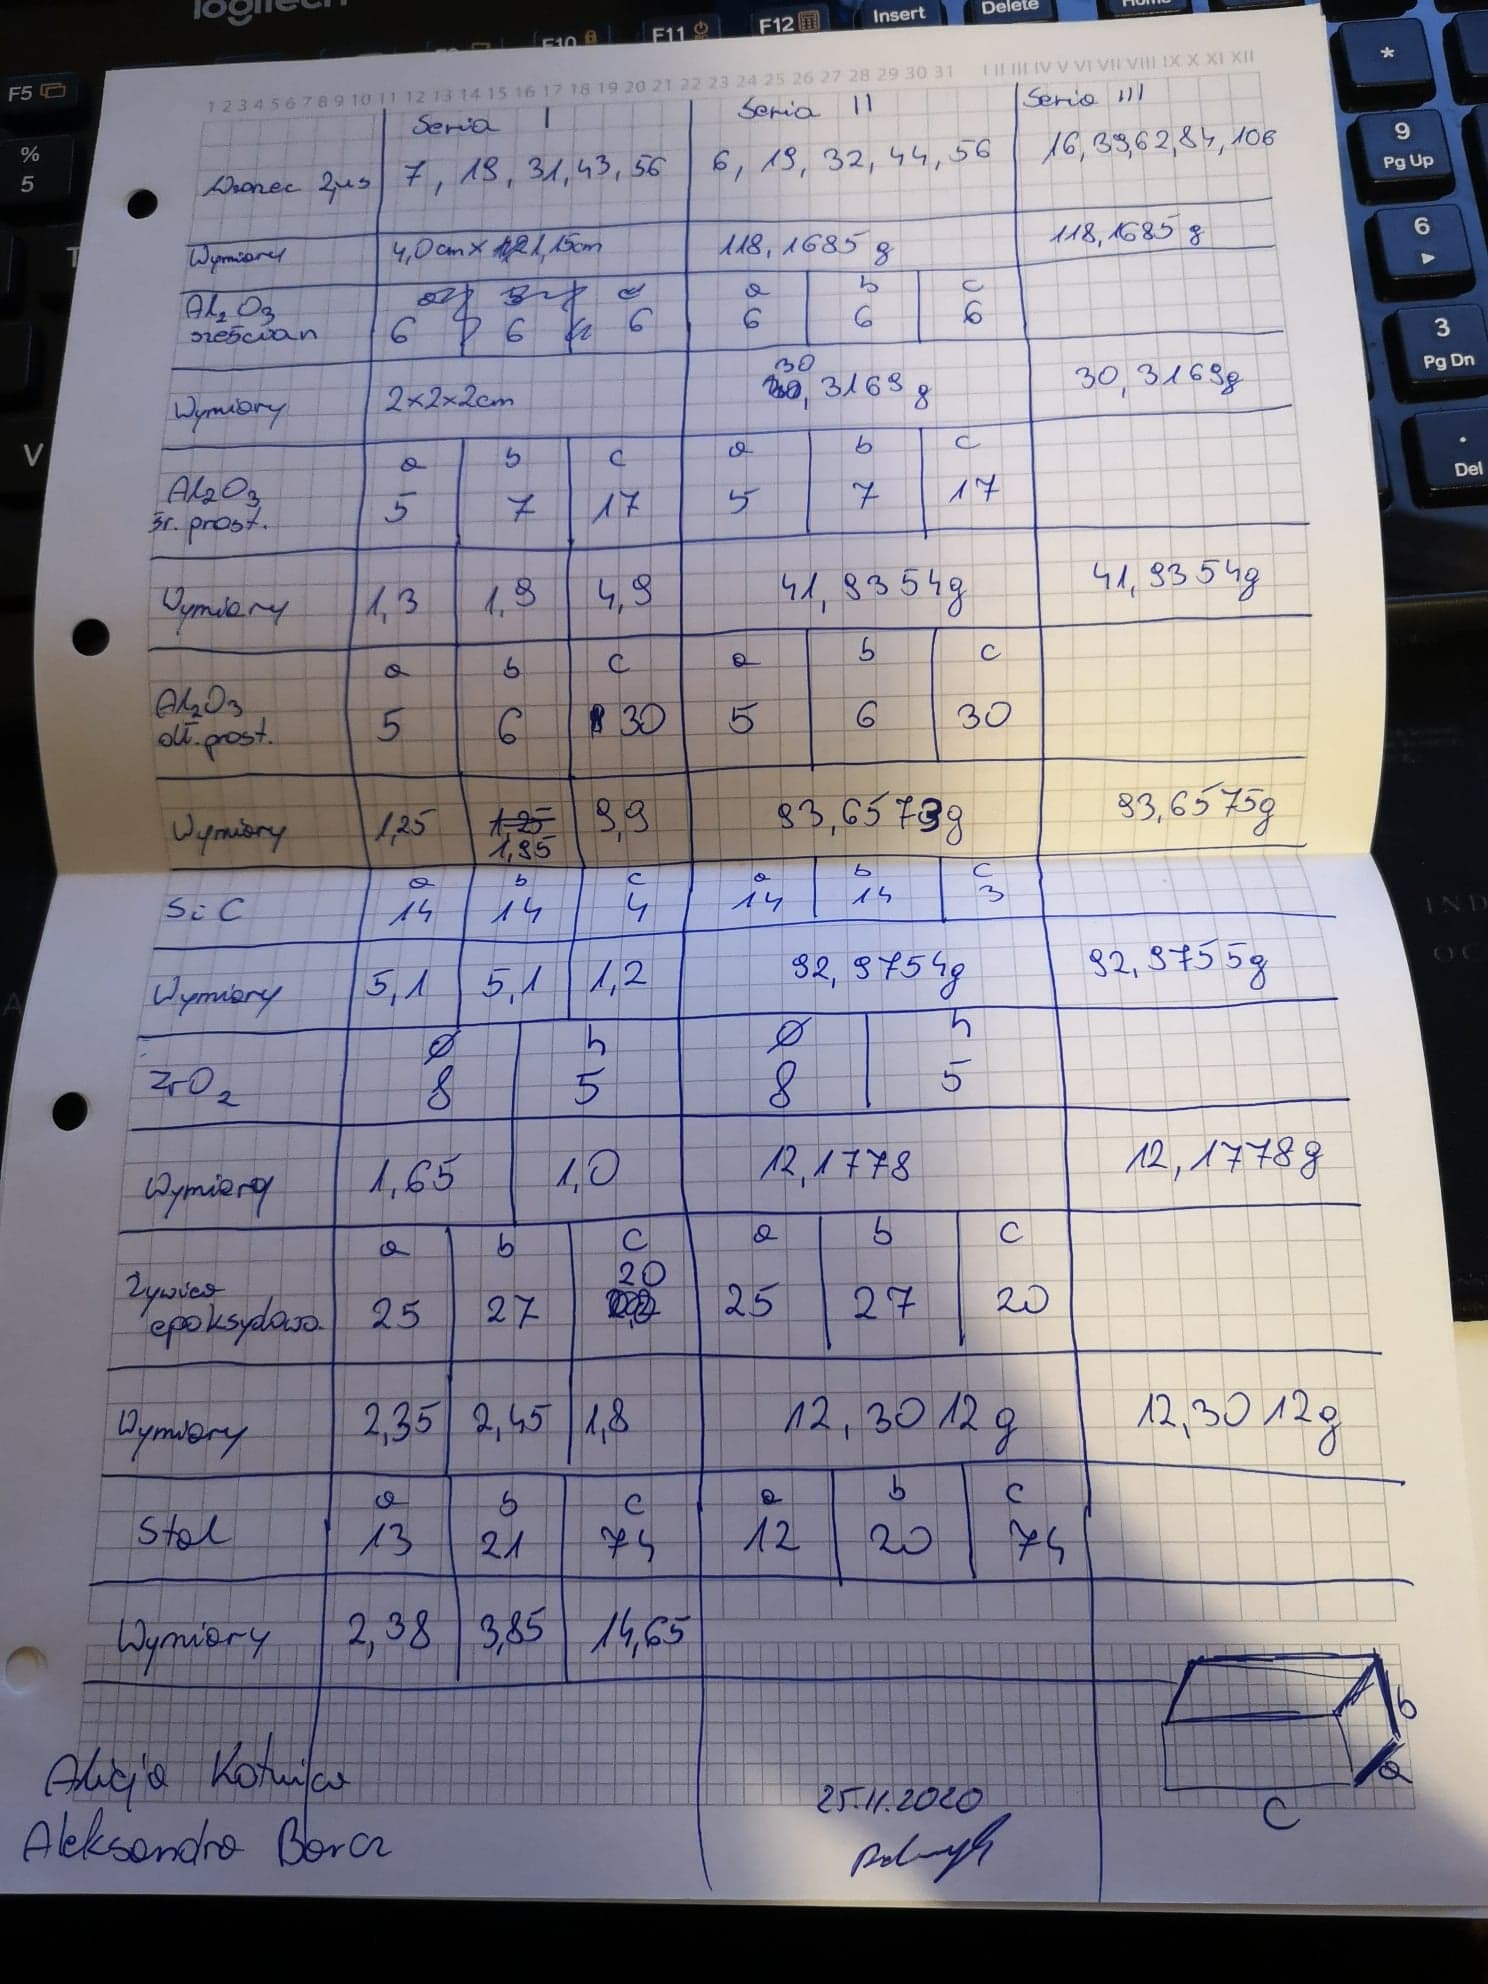
\includegraphics[width=0.7\textwidth]{img/fala_podluzna.jpg}
    \caption{Wyniki pomiarów fali podłużnej oraz zbadane wymiary i~wagi próbek.}
\end{figure}

\begin{figure}[H]
    \centering
    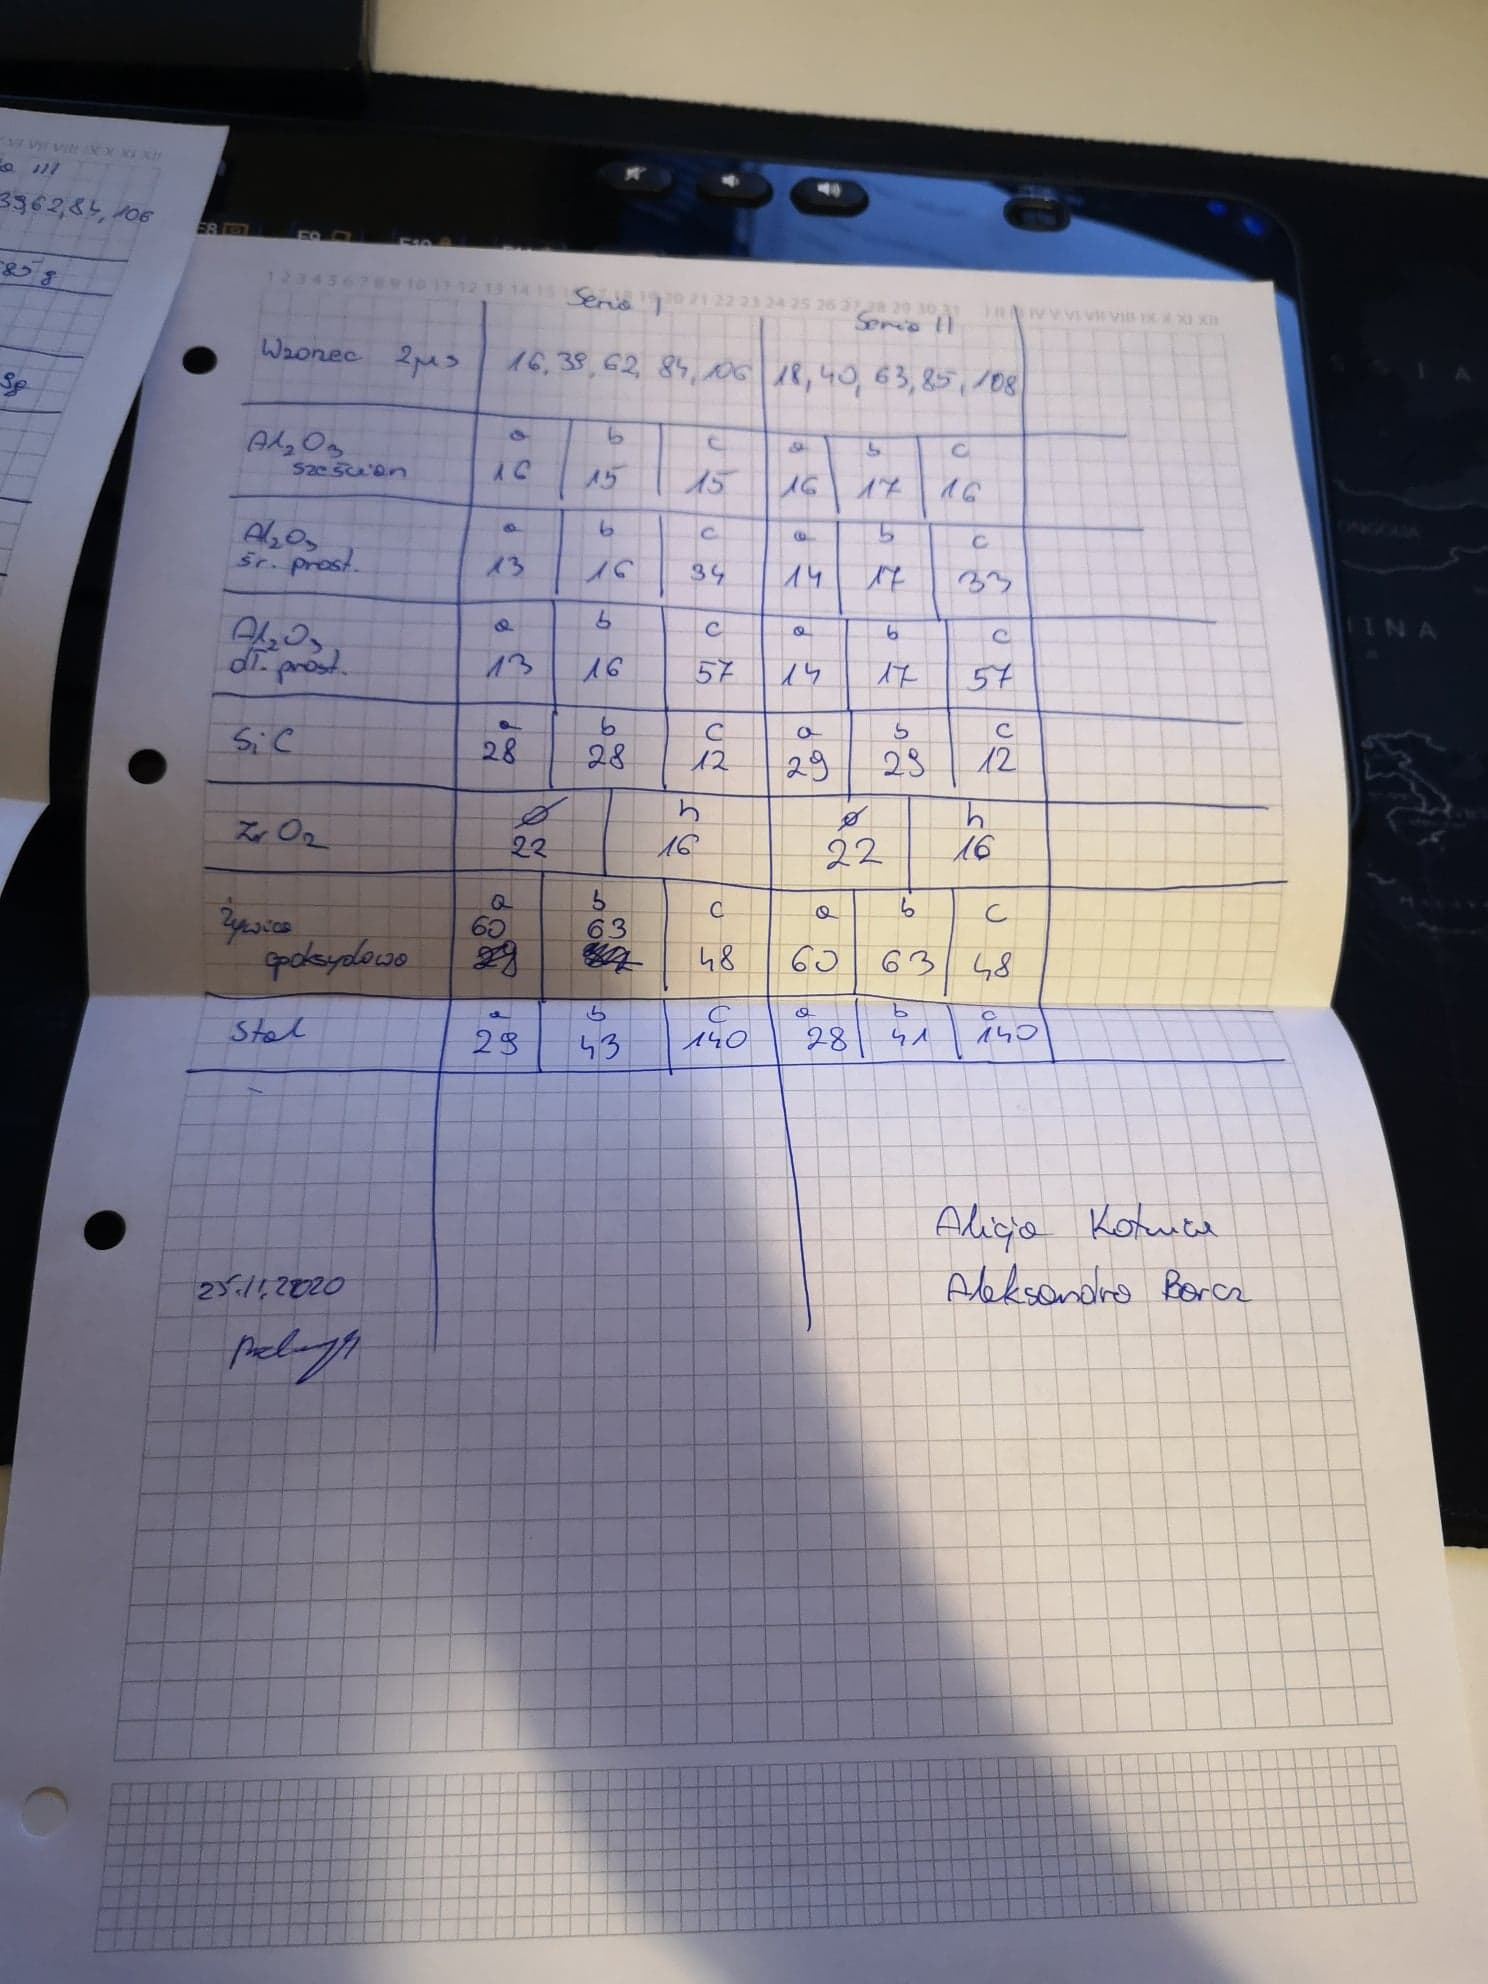
\includegraphics[width=0.7\textwidth]{img/fala_poprzeczna.jpg}
    \caption{Wyniki pomiarów fali poprzecznej.}
\end{figure}

\end{document}
